\section{Datenbankmodelle}
\label{datenmodelle}
In diesem Abschnitt werden die Grundlagen des Graph-basierten Datenbankmodells skizziert. Dieses Graphmodell ist im Rahmen dieser Arbeit von wesentlicher Bedeutung. Schließlich vereint die in \autoref{db2graph} beschriebene Grapherweiterung Elemente des relationalen und Graph-basierten Datenbankmodells. Grundkenntnisse über das relationale Modell werden im Rahmen dieser Arbeit vorausgesetzt. Sollten keine Grundkenntnisse über relationale Datenbanksysteme vorhanden sein, empfehlen sich \cite{rdbms_book} und \cite{codd_relational_model} als Einstieg.

Um die Grundlagen des Graphmodells in diesem Abschnitt zu vermittelen, werden die folgenden Aspekte des Modells angesprochen:
\begin{itemize}
    \item Herkunft und Verbreitung,
    \item Struktur und Schema.
\end{itemize}
Die Beschränkung auf diese Aspekte wurde vorgenommen, da die Erläuterung weiterer Aspekte über den Rahmen dieser Arbeit hinausgehen würde. Anschließend findet eine kurze Gegenüberstellung des Graphmodells mit dem relationalen Modell statt. Zum Schluss werden die Informationen nochmals kurz zusammengefasst. 

\subsection{Herkunft und Verbreitung}
Das Graphmodell als Datenbankmodell hat seinen Ursprung in der heutigen Form im Jahr 1999 \cite{gdbms}. Laut \cite{gdbms} wurde das Graphmodell dabei mit der Motivation entwickelt, Nachteile und Probleme des relationalen Modells auszuräumen. 

Graphdatenbanksysteme und das Graphmodell sind heute als vergleichbar junge Technologien noch nicht so weit verbreitet wie beispielsweise das relationale Modell. Mit 1,7 \% der Ranking-Punkte in \cite{db_engines_ranking_july} ordnen sich Graphdatenbanksysteme dabei noch weit hinter anderen Technologien ein, wie \textit{Document Stores}, \textit{Key-Values Stores} oder \textit{Wide column stores} (\autoref{fig:dbms_marketshare}) \cite{db_engines_ranking_july}. Jedoch haben Graphdatenbanksysteme seit 2013 laut \cite{db_engines_ranking_july} einen erheblichen Aufschwung in ihrer Popularität erfahren. So hat sich der Popularitätsscore dieser Datenbanksystemkategorie im Zeitraum von 01.2013 bis 07.2021 verhundertfacht \cite{db_engines_ranking_july}. 

\begin{figure}[ht]
    \centering
    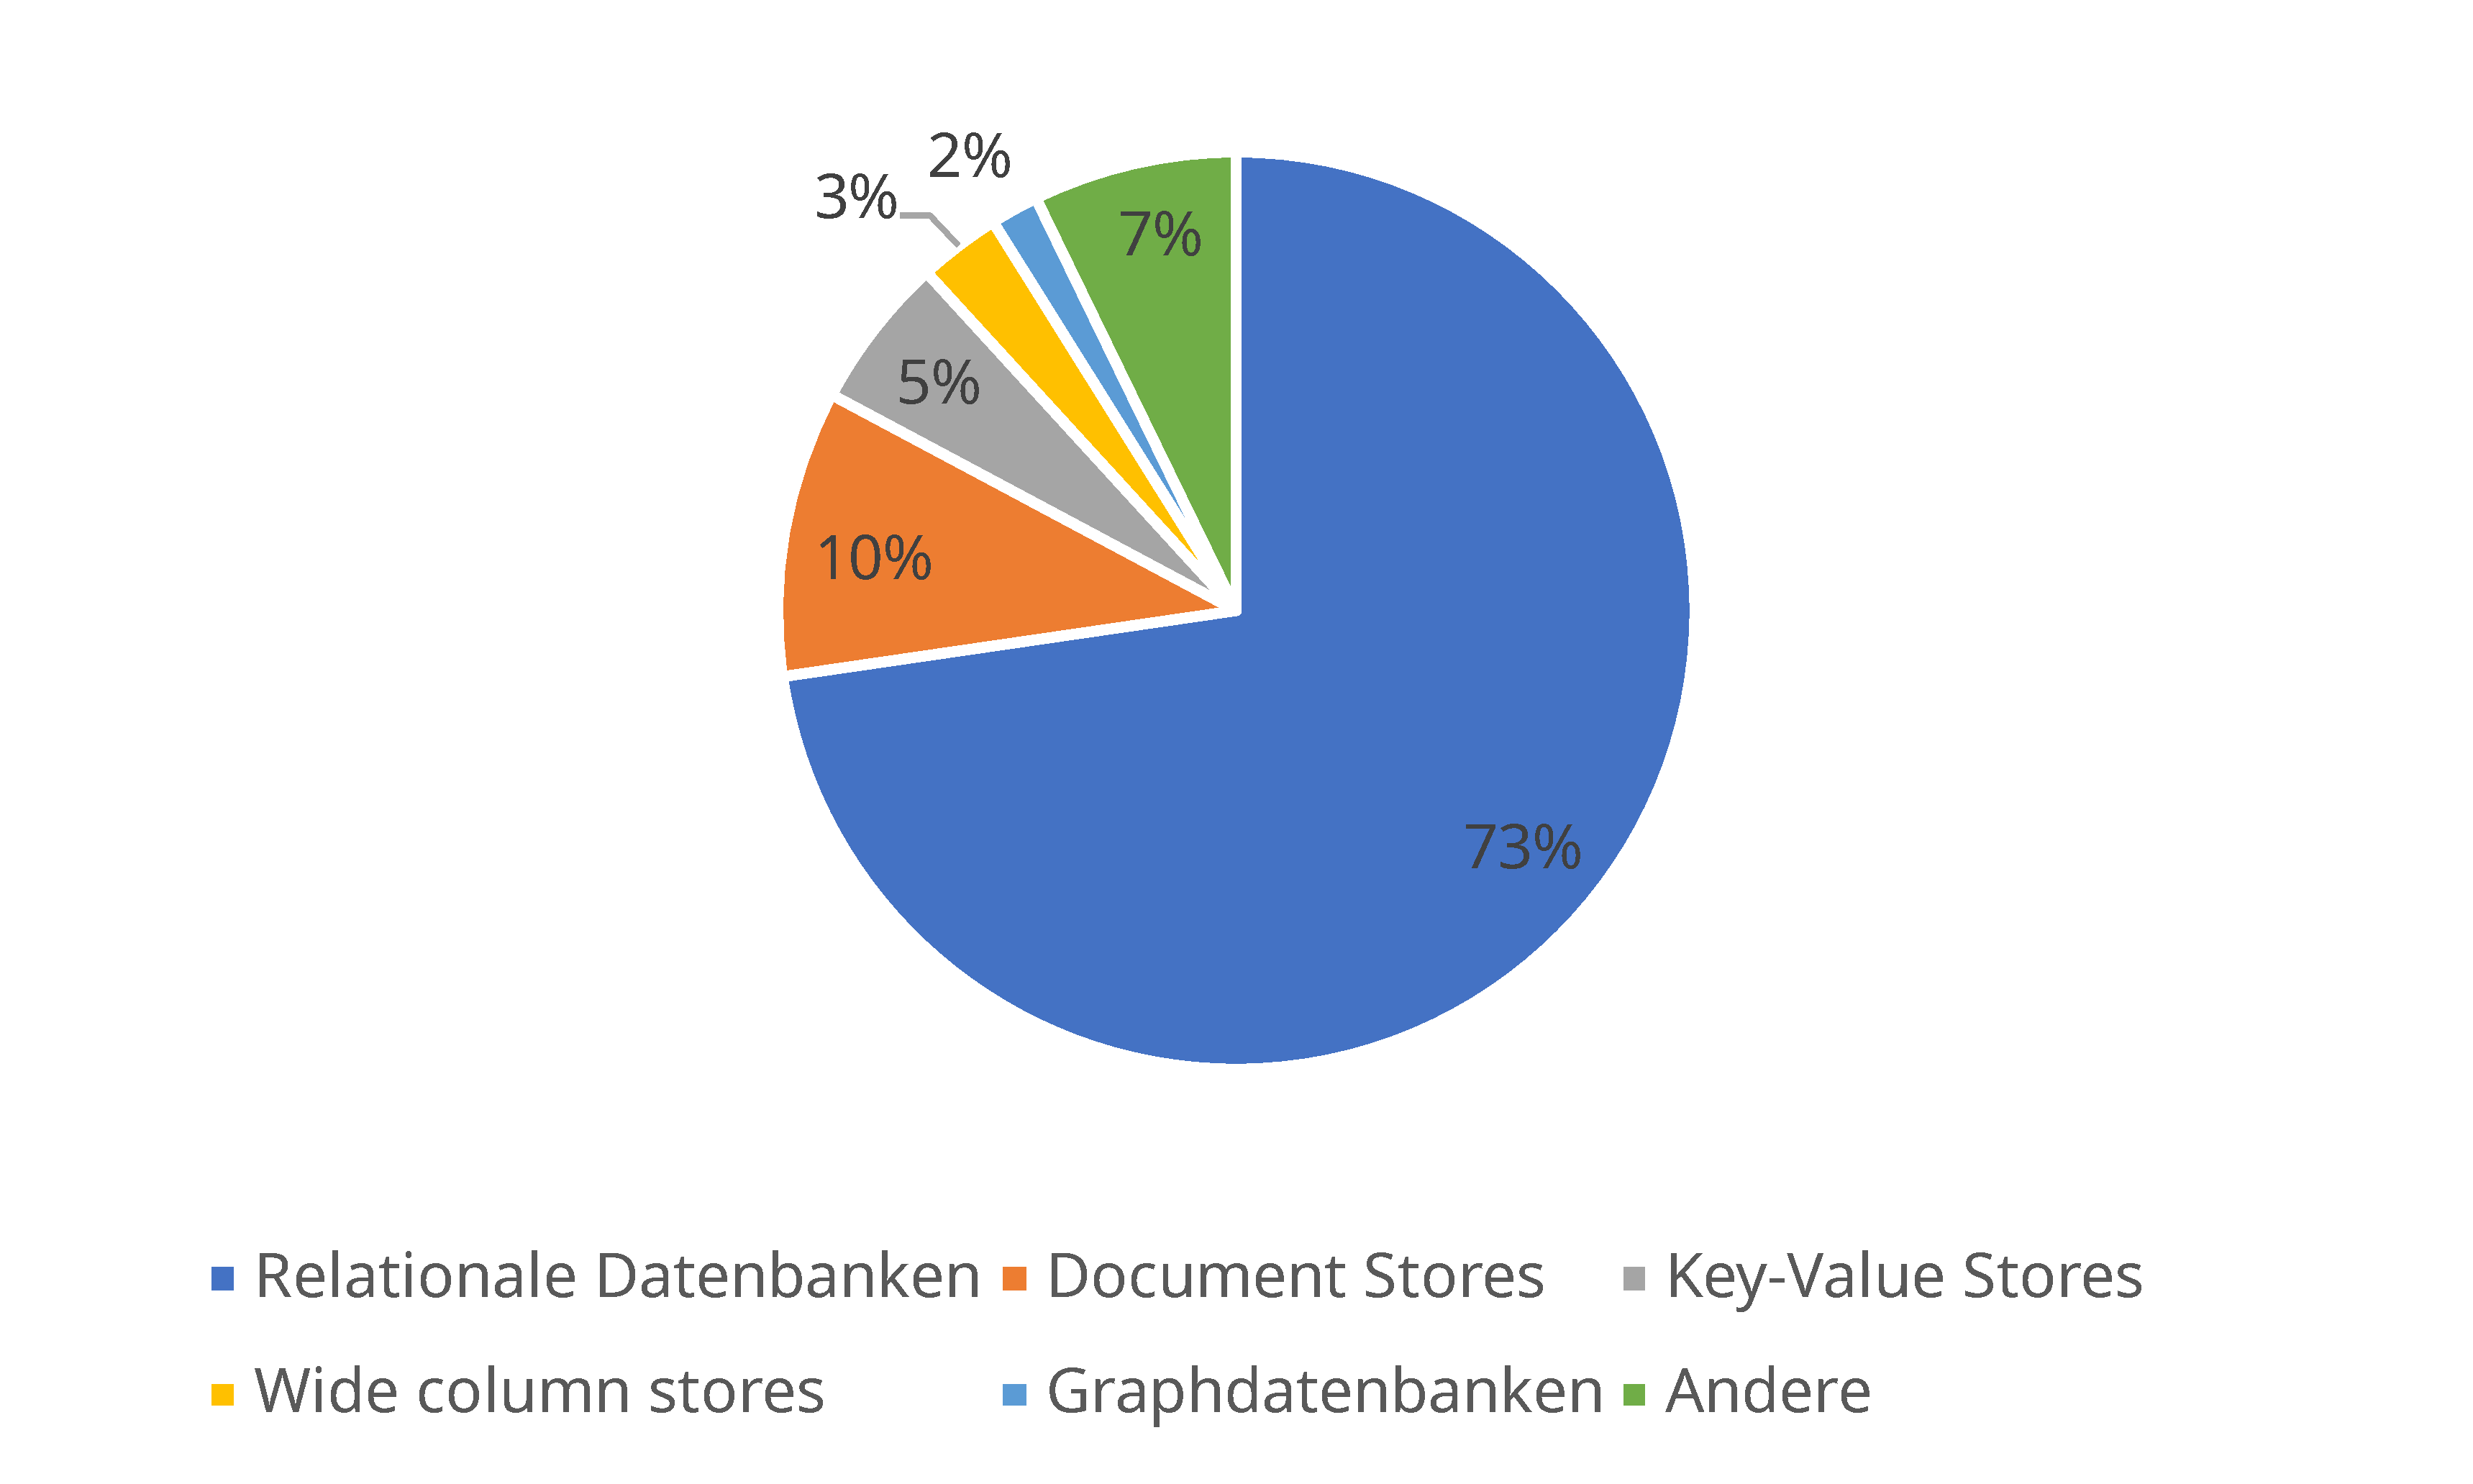
\includegraphics[width=\textwidth]{images/dbms_marketshare.pdf}
    \caption[Anteil Ranking-Punkte nach Datenbankkategorie]{Anteil an Ranking-Punkten nach Datenbankkategorie}
    \label{fig:dbms_marketshare}
    \vspace{1em}
    \textit{Bei den hier abgebildeten Werten handelt es sich um die aufgerundeten Werte aus} \cite{db_engines_ranking_july}\textit{.}
\end{figure}

\subsection{Struktur und Schema}
\label{datenmodelle:structure}
Die Grundlage des Graphmodells stellen sogenannte Knoten (\textit{engl. Vertices oder Vertexes}) und Kanten (\textit{engl. Edges}) dar. Bei einem Graphen handelt es sich hierbei um eine Menge an Knoten und Kanten \cite{gdbms}. In einem solchen Graphen werden dabei Entitäten als Knoten repräsentiert, wie zum Beispiel \textit{Robin} oder \textit{ID3} (\autoref{fig:beispiel_graph}). Die Kanten repräsentieren hingegen, in welcher Beziehung diese Entitäten zueinander stehen. Dies lässt sich exemplarisch an den Kanten \textit{besitzt}, \textit{besaß} oder \textit{kennt} nachvollziehen (\autoref{fig:beispiel_graph}). Wie in \autoref{fig:beispiel_graph} auch erkennbar ist, verfügen die Kanten dabei immer über eine Richtung. Also einen Start- und einen Zielknoten den sie verbinden. 

Knoten und Kanten können dabei in diesem Modell anhand von sogenannten Labels organisiert werden. So können Knoten oder Kanten, die eine ähnliche Rolle einnehmen, dieselben Labels zugewiesen werden. Die Verwendung von Labels wird hierbei in \autoref{fig:beispiel_graph} durch die unterschiedlichen Farben gekennzeichnet. So werden darin die als Auto gelabelten Knoten hellbraun markiert, während die Personen rot eingefärbt werden. 

Das Graphmodell setzt, anders als das relationale Modell, auf ein flexibles Datenbankschema \cite{gdbms}. Durch dieses flexible Schema fällt es leicht, heterogene Daten in dem Graphmodell abzubilden. 

\begin{figure}[ht]
    \centering
    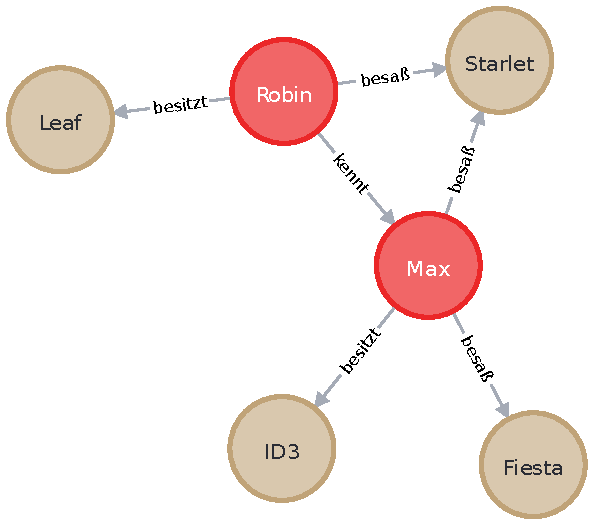
\includegraphics[width=0.75\textwidth]{images/example_graph.pdf}
    \caption{Beispiel Graph}
    \vspace{1em}
    \textit{Hier wird ein Beispiel Graph abgebildet der die Besitzbeziehungen zwischen einer Person (Besitzer) und einem Auto modelliert.}
    \label{fig:beispiel_graph}
\end{figure}

\subsection{Vergleich}
In diesem Unterabschnitt findet ein kurzer Vergleich zwischen dem Graph-basierten und relationalen Datenmodell statt. Dieser kann als kurze Übersicht angesehen werden, der die wichtigsten Unterschiede zwischen den Datenbankmodellen aufführt. 

In der folgenden Aufzählung werden dabei die drei wichtigsten Unterschiede zwischen den Datenmodellen angesprochen:
\begin{itemize}
    \item Das Graphmodell verfügt über ein flexibles Schema, während bei dem relationalen Modell auf ein striktes Schema gesetzt wird \cite{gdbms,rdbms_book}.
    \item Im relationalen Modell werden alle Informationen in Tabellen abgelegt \cite{rdbms_book}. Im Graphmodell werden die Daten in Knoten und Kanten gehalten \cite{gdbms}. 
    \item Beziehungen werden in einem Graphdatenbanksystem durch Kanten zwischen einem Start- und Zielknoten repräsentiert \cite{gdbms}. Beim relationalen Modell werden Beziehungen durch die Referenzierung eines Primärschlüssels einer anderen Tabelle vorgenommen \cite{rdbms_book}. 
\end{itemize}
Bei der genaueren Betrachtung der Unterschiede aus der vorausgegangenen Aufzählung fällt auf, dass diese auch als Ähnlichkeiten betrachtet werden können. So verfügen beide Modelle trotz ihrer unterschiedlichen Herangehensweise über ein Schema, besitzen Strukturen, in denen Informationen gehalten werden und bieten die Möglichkeit, Beziehungen abzubilden. Somit scheinen die beiden Modell zumindest bezüglich dieser Aspekte äquivalent zu sein. Schließlich verfügen beide Datenmodelle über Strukturen und Mechanismen, um Daten zu halten und Beziehungen zu modellieren. 

Wenn nun allerdings beide Datenmodelle über die Mittel verfügen, Daten zu halten und Beziehungen abzubilden, stellt sich die Frage: \textit{Wann sollte welches Datenmodell herangezogen werden?}

Die ausführliche Beantwortung dieser Frage würde hierbei den Rahmen der Arbeit sprengen. Allerdings können die beiden folgenden Szenarien und die abschließenden Anmerkungen kleine Einblicke dazu geben. 

\subsubsection{Szenario 1.}
In diesem Szenario wird auf Queries eingegangen, bei denen Beziehungen beziehungsweise der Beziehungsgrad eine wichtige Rolle spielen. 

Hierfür wird beispielhaft die Angestelltenhierarchie eines Unternehmens herangezogen. Bei den Daten, die die Modelle hierbei repräsentieren sollen, handelt es sich um einen Datensatz an Angestellten. Diese Angestellten verfügen dabei wie in \autoref{fig:angestellten_graph} und \autoref{fig:angestellten_tabelle} erkennbar über einen Namen und einen Vorgesetzten, dem sie unterstellt sind. 

Nun soll in diesem Szenario ermittelt werden, wer \textit{Alice} Vorgesetzter dritten Grades in diesem Unternehmen ist. Also wer der Vorgesetzte des Vorgesetzten des Vorgesetzten von \textit{Alice} ist. Bei dem Graphen in \autoref{fig:angestellten_graph} kann dies leicht nachvollzogen werden. Es muss lediglich dreimal den \texttt{hat\_vorgesetzten}-gelabelten Kanten gefolgt werden, bis der Zielknoten \textit{Dave} erreicht wird. 

\begin{figure}[ht]
    \centering
    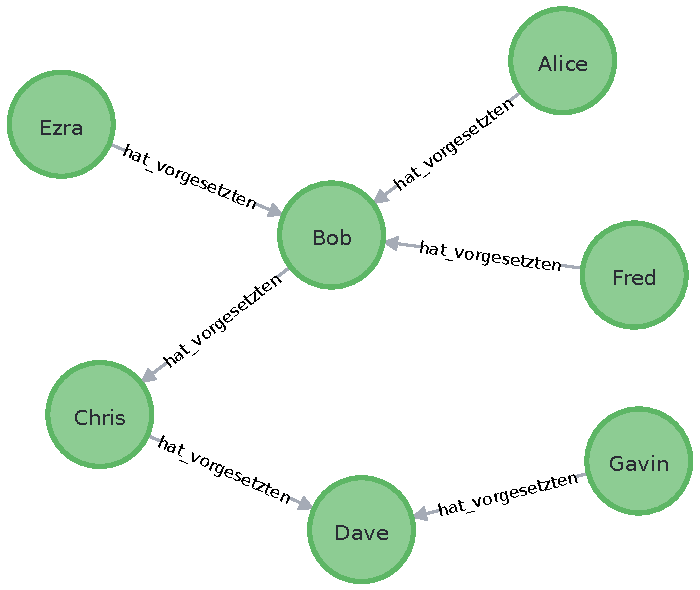
\includegraphics[width=0.8\textwidth]{images/angestellten_graph.pdf}
    \caption{Angestelltenhierarchie Graph}
    \label{fig:angestellten_graph}
\end{figure}

Bei dem in \autoref{fig:angestellten_tabelle} dargestellten Modell ist der Aufwand jedoch etwas höher. Hier müssen zur Ermittlung des Namens des Vorgesetzten dritten Grades mindestens zwei Joins der Tabelle mit sich selbst durchgeführt werden. Dies stellt bei den kleinen Tabellen und dem niedrigen Grad im Anwendungsfall noch kein Problem dar. Bei einem größeren Datensatz oder einem höheren Grad würden beide Faktoren die Last und Performance des Datenbanksystems stark beeinträchtigen. Schließlich sind solche rekursiven Joins Ressourcen-intensiv, besonders wenn zwei große Tabellen gejoined werden \cite{gdbms}. 

\begin{figure}[ht]
    \centering
    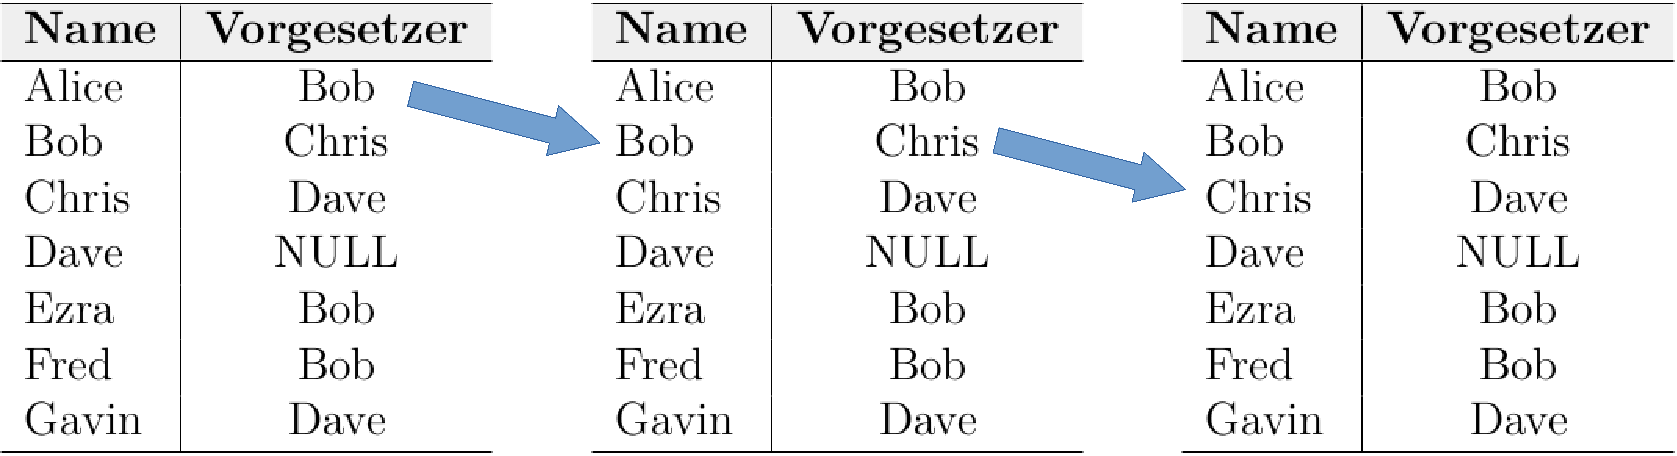
\includegraphics[width=\textwidth]{images/angestellte_tabellen.pdf}
    \caption{Angestelltenhierarchie Tabelle}
    \label{fig:angestellten_tabelle}
\end{figure}

\subsubsection{Szenario 2.}
In diesem Szenario wird auf die Modellierung von heterogenen Daten im Rahmen der beiden Datenmodelle eingegangen. Dafür wird in diesem Szenario versucht, ein Inventar an Küchengeräten und ihre dazugehörigen Küchen mit den jeweiligen Modellen abzubilden. 

\autoref{tab:kaffeemaschinen} bis \autoref{tab:kuechen} stellen dabei die Tabellen dar, die für die Abbildung der verschiedenen Küchengeräte und jeweiligen Küchen im relationalen Modell erforderlich sind. Dabei fällt auf, dass für die Darstellung von zehn Küchengeräten acht verschiedene Tabellen benötigt werden. Schließlich handelt es sich bei den Küchengeräten um heterogene Daten, welche für die Erfassung aller Merkmale im strikten Schema des relationalen Modells, eine solche Handhabung erfordern. 

Diese Vielzahl an Tabellen sorgt dafür, dass sich beispielsweise die Abfrage aller Geräte, die zur Küche von \textit{Alice} gehören, sehr kompliziert gestaltet. Denn bei einem solchen Prozess müssen viele verschiedene Tabellen miteinander gejoined werden. Daher kann daraus geschlossen werden, dass sich das relationale Modell nicht für die Modellierung solcher heterogenen Daten eignet.

\begin{table}[!ht]
    \centering
    \begin{tabular}{c|c|r|c|c}
    \hline
    \rowcolor[HTML]{EFEFEF} 
    \textbf{Gerätenummer} & \textbf{Hersteller} & \multicolumn{1}{c|}{\cellcolor[HTML]{EFEFEF}\textbf{Baujahr}} & \textbf{Vollautomat} & \textbf{Küche} \\ \hline
    Jura-123 & Jura & 2012 & TRUE & 1 \\
    Delonghi-456 & Delonghi & 2019 & FALSE & 2 \\ \hline
    \end{tabular}
    \caption{Kaffeemaschinen}
    \label{tab:kaffeemaschinen}
\end{table}

\begin{table}[!ht]
    \centering
    \begin{tabular}{c|c|c|c|c}
    \hline
    \rowcolor[HTML]{EFEFEF} 
    \textbf{Gerätenummer} & \textbf{Hersteller} & \textbf{Baujahr} & \textbf{Grillfunktion} & \textbf{Küche} \\ \hline
    Bosch-1000 & Bosch & \multicolumn{1}{r|}{2013} & TRUE & 1 \\ \hline
    \end{tabular}
    \caption{Mikrowellen}
    \label{tab:mikrowellen}
\end{table}

\begin{table}[!ht]
    \centering
    \begin{tabular}{c|c|c|c}
    \hline
    \rowcolor[HTML]{EFEFEF} 
    \textbf{Gerätenummer} & \textbf{Hersteller} & \textbf{Baujahr} & \textbf{Küche} \\ \hline
    Tefal-100 & Tefal & \multicolumn{1}{r|}{2020} & 2 \\ \hline
    \end{tabular}
    \caption{Fritteusen}
    \label{tab:fritteuse}
\end{table}

\begin{table}[!ht]
    \centering
    \begin{tabular}{c|c|r|r|c}
    \hline
    \rowcolor[HTML]{EFEFEF} 
    \textbf{Gerätenummer} & \textbf{Hersteller} & \multicolumn{1}{c|}{\cellcolor[HTML]{EFEFEF}\textbf{Baujahr}} & \multicolumn{1}{c|}{\cellcolor[HTML]{EFEFEF}\textbf{Max. Temp. in °C}} & \textbf{Küche} \\ \hline
    Miele-365 & Miele & 2010 & 250 & 2 \\
    AEG-200 & AEG & 2013 & 300 & 1 \\ \hline
    \end{tabular}
    \caption{Backöfen}
    \label{tab:backoefen}
\end{table}

\begin{table}[!ht]
    \centering
    \begin{tabular}{c|c|r|c|c}
    \hline
    \rowcolor[HTML]{EFEFEF} 
    \textbf{Gerätenummer} & \textbf{Hersteller} & \multicolumn{1}{c|}{\cellcolor[HTML]{EFEFEF}\textbf{Baujahr}} & \textbf{Gefrierfach} & \textbf{Küche} \\ \hline
    Liebherr-1 & Liebherr & 2015 & TRUE & 1 \\
    Liebherr-2 & Liebherr & 2017 & FALSE & 2 \\ \hline
    \end{tabular}
    \caption{Kühlschränke}
    \label{tab:kuehlschraenke}
\end{table}

\begin{table}[!ht]
    \centering
    \begin{tabular}{c|c|c|c|c}
    \hline
    \rowcolor[HTML]{EFEFEF} 
    \textbf{Gerätenummer} & \textbf{Hersteller} & \textbf{Baujahr} & \textbf{Füllmenge in l} & \textbf{Küche} \\ \hline
    Unold-1 & Unold & \multicolumn{1}{r|}{2017} & 1,5 & 2 \\ \hline
    \end{tabular}
    \caption{Brotbackautomaten}
    \label{tab:brotbackautomaten}
\end{table}

\begin{table}[!ht]
    \centering
    \begin{tabular}{c|c|c|c|c|c}
    \hline
    \rowcolor[HTML]{EFEFEF} 
    \textbf{\begin{tabular}[c]{@{}c@{}}Geräte-\\ nummer\end{tabular}} & \textbf{Hersteller} & \textbf{Baujahr} & \textbf{\begin{tabular}[c]{@{}c@{}}Füllmenge\\ in Liter\end{tabular}} & \textbf{\begin{tabular}[c]{@{}c@{}}Dampfgar-\\ funktion\end{tabular}} & \textbf{Küche} \\ \hline
    Zojirushi-1 & Zojirushi & \multicolumn{1}{r|}{2008} & 1 & FALSE & 2 \\ \hline
    \end{tabular}
    \caption{Reiskocher}
    \label{tab:reiskocher}
\end{table}

\begin{table}[!ht]
    \centering
    \begin{tabular}{c|c}
    \hline
    \rowcolor[HTML]{EFEFEF} 
    \textbf{Nummer} & \textbf{Besitzer} \\ \hline
    1 & Alice \\
    2 & Bob \\ \hline
    \end{tabular}
    \caption{Küchen}
    \label{tab:kuechen}
\end{table}

Die in \autoref{fig:kuechen_graph} dargestellte Repräsentation der Küchen und Küchengeräte in einem Graphmodell zeigt hingegen, dass sich das Graphmodell für die Haltung heterogener Daten eignet. Schließlich muss hierbei lediglich den eingehenden \textit{gehört}-Kanten gefolgt werden, wenn ermittelt werden soll, welche Küchengeräte alle zur Küche von \textit{Alice} gehören.

\begin{figure}[ht]
    \centering
    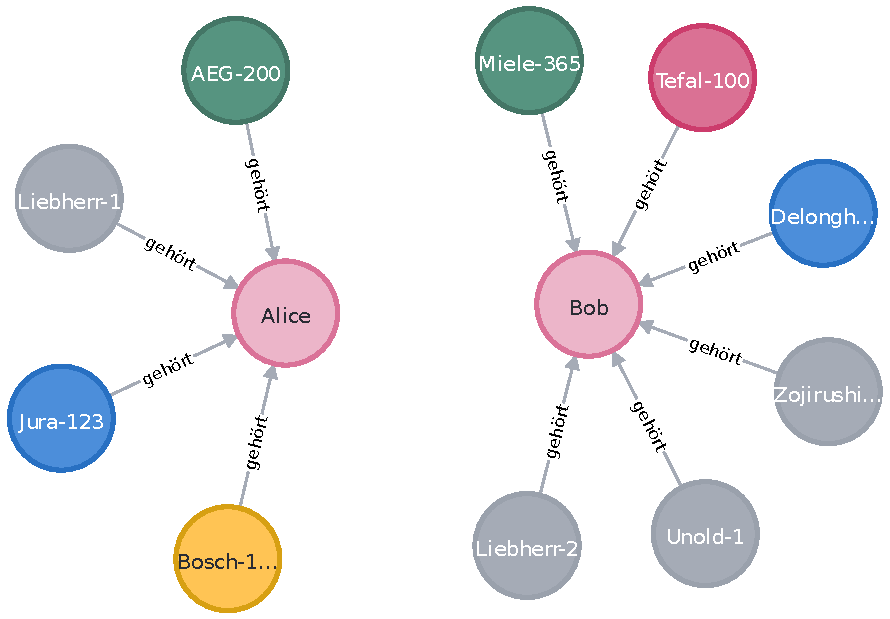
\includegraphics[width=0.8\textwidth]{images/kuechen_graph.pdf}
    \caption{Küchen Graph}
    \label{fig:kuechen_graph}
\end{figure}

\subsubsection{Anmerkungen}
Auch wenn die beiden zuvor aufgeführten Szenarien hier die Vorteile des Graphmodells betonten, so können alle Szenarien auch mit dem relationalen Modell abgebildet werden. 

Des Weiteren gilt es darauf hinzuweisen, dass die Softwareentwicklung für ein relationales Datenbanksystem in einigen Fällen mit weniger Entwicklungsaufwand als bei dem Graphmodell verbunden sein kann. Denn wenn auch in Szenario 2. mehrere Tabellen für die Abbildung der Küchengeräte benötigt werden, so ist bei der Abfrage eines Eintrags aus einer dieser Tabellen immer gesichert, dass er über Werte für die als Spalten definierten Eigenschaften verfügt. Bei Datenbanken, die auf dem Graphmodell basieren, ist dies nicht automatisch gesichert. Hier können Knoten mit denselben Labels unterschiedliche Eigenschaften und Werte aufweisen. So muss die entwickelte Software mit diesen heterogenen Daten umgehen können. Daraus ergibt sich jedoch meist ein höherer Entwicklungsaufwand. 

\subsection{Zusammenfassung}
Bei dem Graphmodell und Graphdatenbanksystemen handelt es sich noch um eine recht junge Technologie, die bisher lediglich eine vergleichsweise kleine Verbreitung gefunden hat. Allerdings scheint sie in den letzten Jahren einen Aufschwung in Popularität erfahren zu haben. 

Die Grundstrukturen des Graphmodells stellen hierbei Knoten und Kanten dar. Diese Strukturen werden dazu herangezogen, Entitäten und ihre Beziehungen zueinander zu repräsentieren. Darüber hinaus setzt das Graphmodell auf ein flexibles Datenbankschema. In diesem werden die Knoten und Kanten anhand von Labels organisiert.

Zwischen dem Graphmodell und relationalen Datenmodell gibt es einige größere Unterschiede, allerdings lassen sich mit beiden Modellen Entitäten und ihre Beziehungen repräsentieren. Dies bedeutet aber nicht, dass sich auch beide Modelle für die Abbildung derselben Daten eignen. So scheint es Szenarien und Anwendungsfälle zu geben, für die sich jeweils eines der Modelle besser eignet. 